\chapter{Desenvolvimento do Trabalho}
\label{cap:desenvolvimento}

Esse capítulo trata do desenvolvimento do trabalho, indicando a metodologia utilizada, a infraestrutura disponível para realização dos testes e ainda o cronograma das atividades propostas. Descreve também os experimentos realizados, com a apresentação dos algoritmos e distribuição dos dados da carga de trabalho.

\section{Metodologia}

A primeira fase do projeto foi destinada ao estudo mais detalhado da computação paralela, em especial dos algoritmos de ordenação paralela, do modelo MapReduce e da plataforma Hadoop. Foram executados testes com os exemplos disponíveis no código do Hadoop e com os \textit{benchmarks} \textit{TeraSort} e \textit{Sort}. 
Após esses testes, foram realizados experimentos com o algoritmo Ordenação por Amostragem, com dados em distribuição uniforme, mesma carga de dados utilizada no trabalho de Pinhão (2011). Além dessa carga de dados, foram feitos testes incluindo duas novas distribuições: Normal e Pareto. 

Os testes buscavam confirmar um funcionamento adequado do algoritmo com diferentes entradas e número de máquinas, além de medir o desempenho dos algoritmos com relação à quantidade de máquinas, quantidade de dados e conjunto de dados. Os resultados obtidos até o momento foram analisados a fim de permitir comparar o desempenho dos algoritmos em cada situação.
 
O passo seguinte foi conhecer detalhadamente o algoritmo paralelo a ser implementado, o \textit{Quicksort}.  No próximo semestre serão definidas as estratégias para sua implementação em ambiente Hadoop e realizados os testes.

\section{Infraestrutura}

A infraestrutura necessária ao desenvolvimento do projeto foi fornecida pelo Laboratório de Redes e Sistemas (LABORES) do Departamento de Computação do Centro Federal de Educação Tecnológica de Minas Gerais (DECOM). O LABORES possui um \textit{cluster} formado por cinco máquinas Dell Optiplex 380, que estão sendo utilizados na realização dos testes dos algoritmos. 

%Os algoritmos serão desenvolvidos em linguagem Java, de acordo com o modelo MapReduce, no ambiente Hadoop. 

Cada máquina do \textit{cluster} apresenta as seguintes características:
\begin{packed_enum}
\item Processador Intel Core 2 Duo de 3.0 GHz
\item Disco rígido SATA de 500 GB 7200 RPM
\item Memória RAM de 4 GB
\item Placa de rede Gigabit Ethernet
\item Sistema operacional Linux Ubunbu 10.04 32 bits %(kernel 2.6.\textbf{XX})
\item Sun Java JDK 1.6.0 19.0-b09 
\item Apache Hadoop 1.0.2
\end{packed_enum}


\section{Descrição dos experimentos}
\label{sec:experimentos}

A primeira parte dos experimentos consistiu em reproduzir os resultados já encontrados no trabalho de referência: testes de ordenação com os \textit{benchmarks TeraSort} e \textit{Sort}, e com o algoritmo Ordenação por Amostragem. 
Em todos os casos, os testes foram compostos de duas partes: geração da carga de dados e ordenação. 

\subsection{Benchmarks: TeraSort e Sort}

%A execução dos \textit{benchmarks} TeraSort e Sort foram os primeiros testes de ordenação realizados. A importância desses testes consiste no fato dessas aplicações de ordenação serem conhecidas e consolidados no ambiente Hadoop. 
 
Para compreender o funcionamento dos algoritmos de ordenação e do ambiente Hadoop foram executados, primeiramente, testes com os \textit{benchmarks} \textit{TeraSort} e \textit{Sort}.  A importância desses testes consiste no fato de tais  aplicações serem conhecidas e consolidados no ambiente Hadoop. 
 O objetivo dos testes foi verificar se as condições do ambiente eram similares às apresentadas no trabalho de Pinhão (2011). Para tal, os parâmetros dos algoritmos e número de máquinas utilizadas foram similares. 

%\subsubsection{Terasort}

O \textit{TeraSort} consiste de três algoritmos, que são responsáveis pela geração dos dados, ordenação e validação, conforme descrito na seção \ref{sec:benchmarks}.
Os testes com o \textit{TeraSort} foram feitos em duas máquinas. Foram gerados pelo \textit{TeraGen} dois arquivos contendo 50 mil linhas cada e o algoritmo foi executado 10 vezes.

 
%A geração dos dados é feita pelo algoritmo TeraGen. O número de registros é um parâmetro definido pelo usuário, e os dados gerados são divididos em dois arquivos. O TeraSort lê os arquivos gerados e realiza a ordenação. Após a ordenação, os dados são validados pelo TeraValidade. Caso haja algum erro na ordenação, o algoritmo escreve um arquivo informando quais foram as chaves com erros.  

%\subsubsection{Sort}

%Sort é um dos \textit{benchmarks}  de ordenação de dados mais conhecidos para Hadoop. Ele é uma aplicação MapReduce, que realiza uma ordenação dos dados de entrada. Além da ordenação, é fornecido um programa padrão para geração de dados aleatórios de entrada, o RandomWriter. 

Para os testes realizados com o \textit{Sort} foram utilizados dados gerados pelo algoritmo \textit{RandomWriter}. Para cada máquina do \textit{cluster}, foram escritos 10 arquivos de 1GB cada em formato binário, totalizando 10GB. Os testes foram feitos em 4 máquinas, com 10 execuções. 


\subsection{Ordenação por Amostragem}

Os experimentos com o algoritmo Ordenação por Amostragem foram divididos em duas fases. A primeira fase consistiu na reprodução dos testes realizados no trabalho de referência, com o algoritmo implementado em Java, no ambiente Hadoop. A segunda fase dos experimentos consistiu em executar o algoritmo em cenários diferentes dos que já haviam sido apresentados. O objetivo de cada experimento era avaliar o algoritmo em situações diversas, confirmando sua escalabilidade e eficiência.

%Foram feitos três tipos de experimentos com o algoritmo, com alterações: (i) no número de arquivos, (ii) no número de máquinas e (iii) carga de dados. Em todos os casos utilizou-se a distribuição uniforme, similar à utilizada no trabalho de Pinhão (2011).

Os experimentos realizados nas duas fases podem ser divididos em três categorias, de acordo com as variações propostas: (i) no número de arquivos e (ii) no número de máquinas. 
O primeiro experimento manteve constante tanto o tamanho do arquivo a ser ordenado quanto o número de máquinas utilizadas na ordenação. 
O segundo experimento manteve constante o número de máquinas utilizadas e variou o tamanho do arquivo a ser ordenado. 
Já o terceiro experimento manteve constante o número de dados e alterou a quantidade de máquinas utilizadas. 

Na primeira fase, foram realizados os três experimentos, e em todos os casos utilizou-se a distribuição uniforme na geração dos dados, similar à utilizada no trabalho de Pinhão (2011). Os arquivos gerados continham entre $10^{6}$ (12MB) e  $10^{10}$ (120GB) chaves, e o número de máquinas utilizadas variou de 2 a 5.
Na segunda fase, cada um dos experimentos foi realizado com três conjuntos diferentes de dados.
Os dados utilizados foram números gerados aleatoriamente em três distribuições: uniforme, normal e pareto. As distribuições foram geradas por um programa implementado em Java para geração de chaves aleatórias de ponto flutuante, contendo entre $10^{6}$ (12MB) e  $10^{10}$ (120GB) chaves. 

As Figuras \ref{fig:uniforme}, \ref{fig:normal} e \ref{fig:pareto} exibem o padrão de frequência das chaves das três distribuições: uniforme, normal e pareto, respectivamente. 
Pode-se observar que as três distribuições tem padrões de comportamento bastante distintos, que se refletem nos arquivos de entrada gerados. A distribuição pareto é a única que está apresentada em escala logarítmica, para melhor visualização. 
Na distribuição uniforme cada chave tem a mesma probabilidade de aparecimento, levando a chaves igualmente distribuídas no intervalo. A distribuição normal concentra grande parte dos valores próximos à media, e distribui poucas chaves em valores mais extremos. A distribuição pareto possui uma grande concentração de chaves em valores próximos de 0, e pequena quantidade de valores mais altos, resultado em valores com baixa frequência no intervalo restante. %Isso pode ser visto pela escala logarítmica utilizada no gráfico que exibe essa distribuição.

\begin{figure}[!h]

\centering
\subfigure[Distribuição Uniforme]{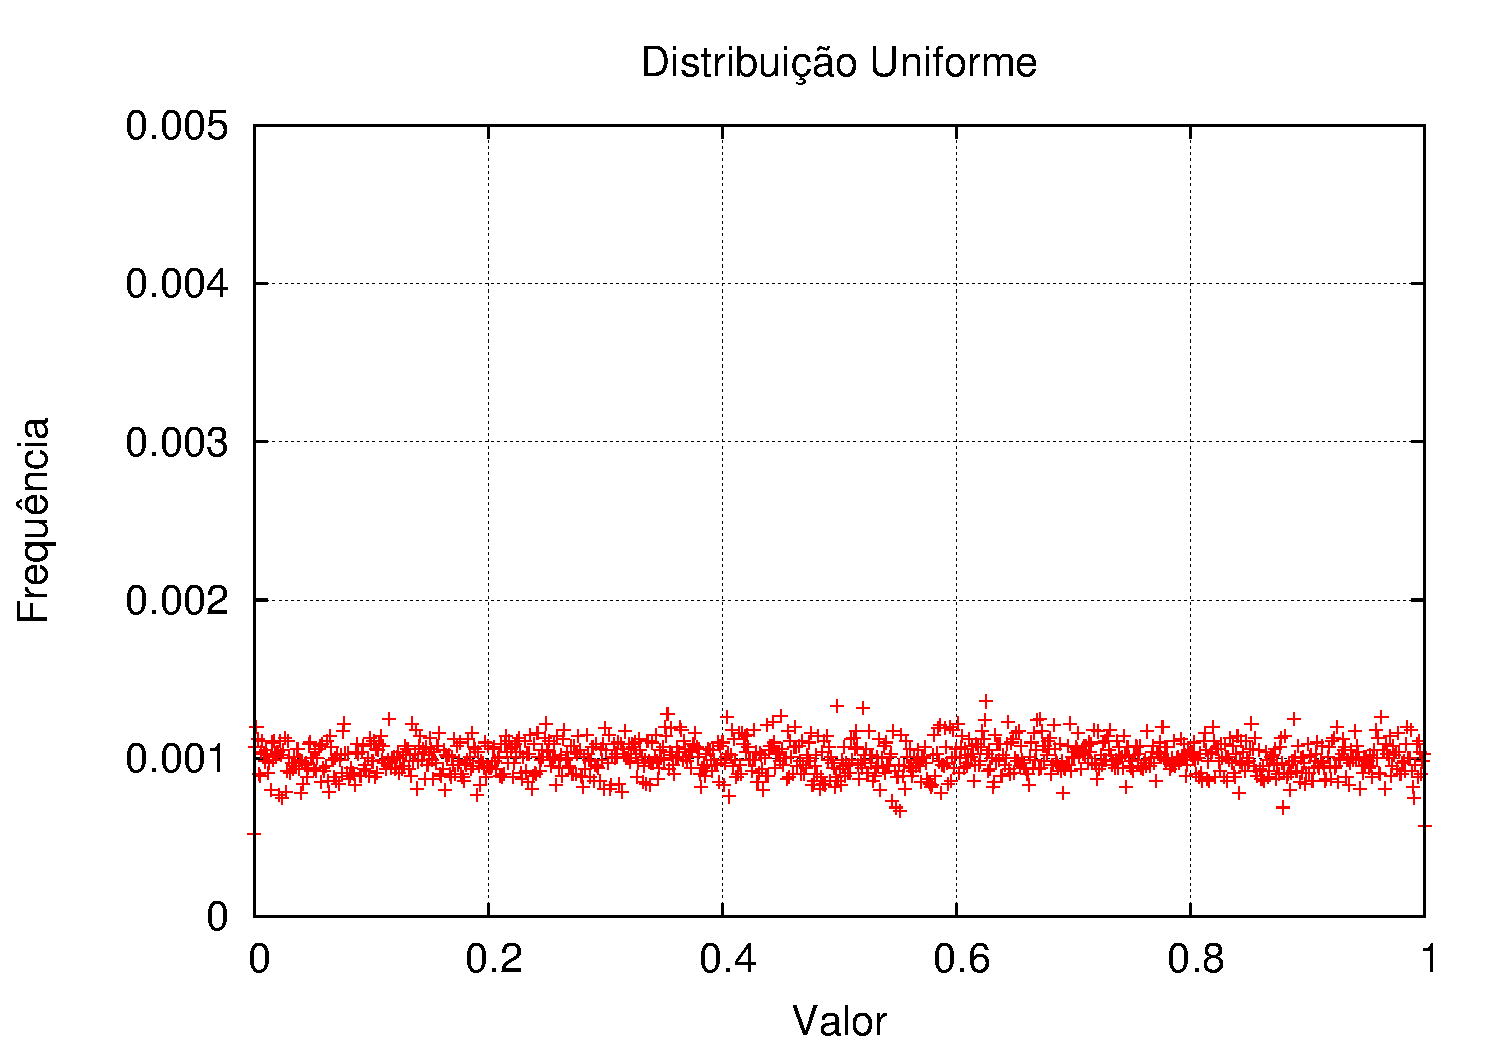
\includegraphics[width=0.48\textwidth]{figuras/DistribuicaoUniforme.pdf} \label{fig:uniforme}}
\qquad
\subfigure[Distribuição Normal]{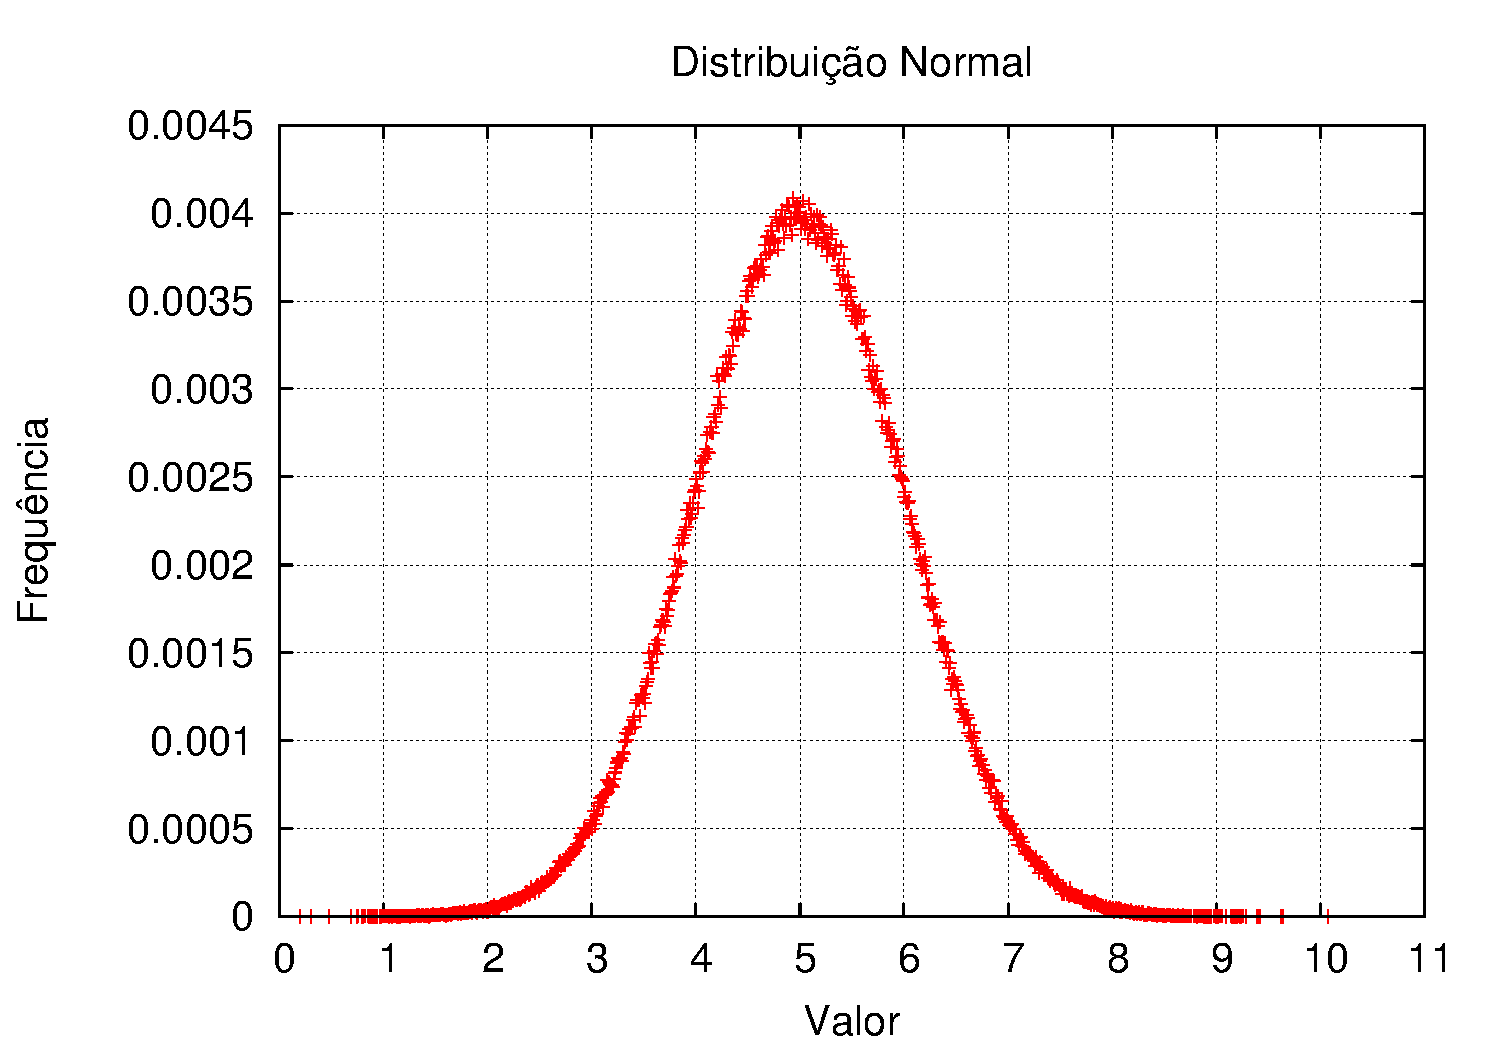
\includegraphics[width=0.48\textwidth]{figuras/DistribuicaoNormal.pdf} \label{fig:normal}}
\subfigure[Distribuição Pareto]{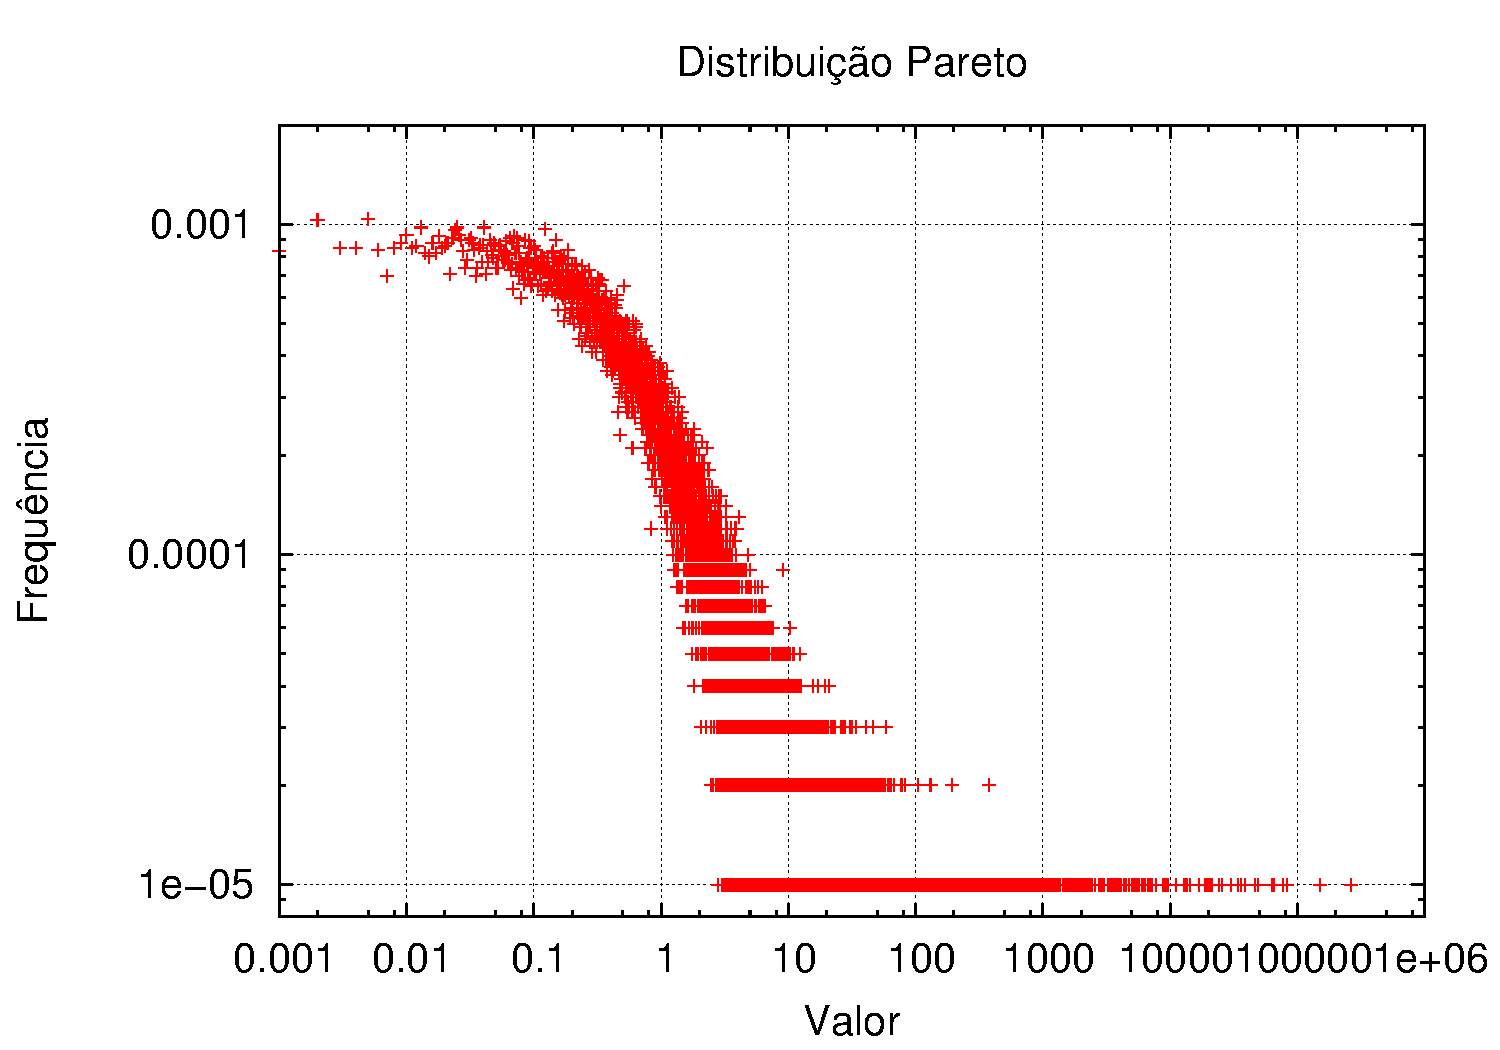
\includegraphics[width=0.48\textwidth]{figuras/DistribuicaoPareto.pdf} \label{fig:pareto}}
\caption{Distribuições dos dados gerados para ordenação}

\end{figure}


% \begin{figure}
% \centering
%%trim left, bottom, right and top [trim=0cm 2cm 0cm 1cm, width=\textwidth]
%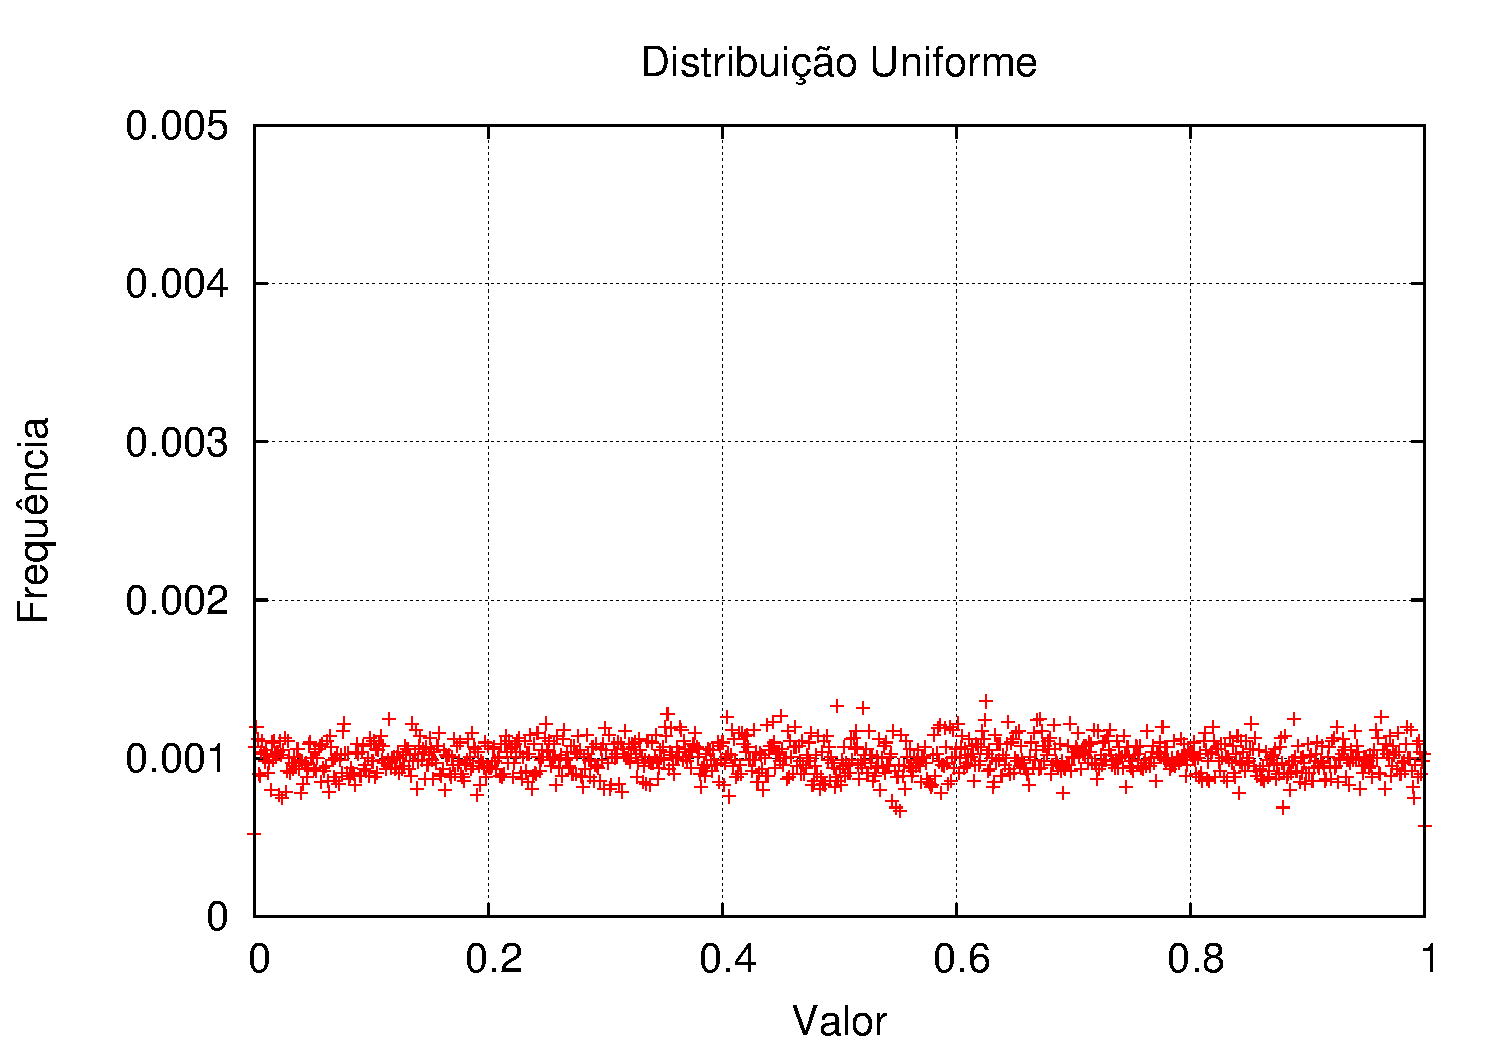
\includegraphics[width=0.3\textwidth]{figuras/DistribuicaoUniforme.pdf}
%\caption{Distribuição Uniforme}
%\label{fig:uniforme}
%\end{figure}
%
%  \begin{figure}
% \centering
%%trim left, bottom, right and top trim=0cm 2cm 0cm 1cm,
%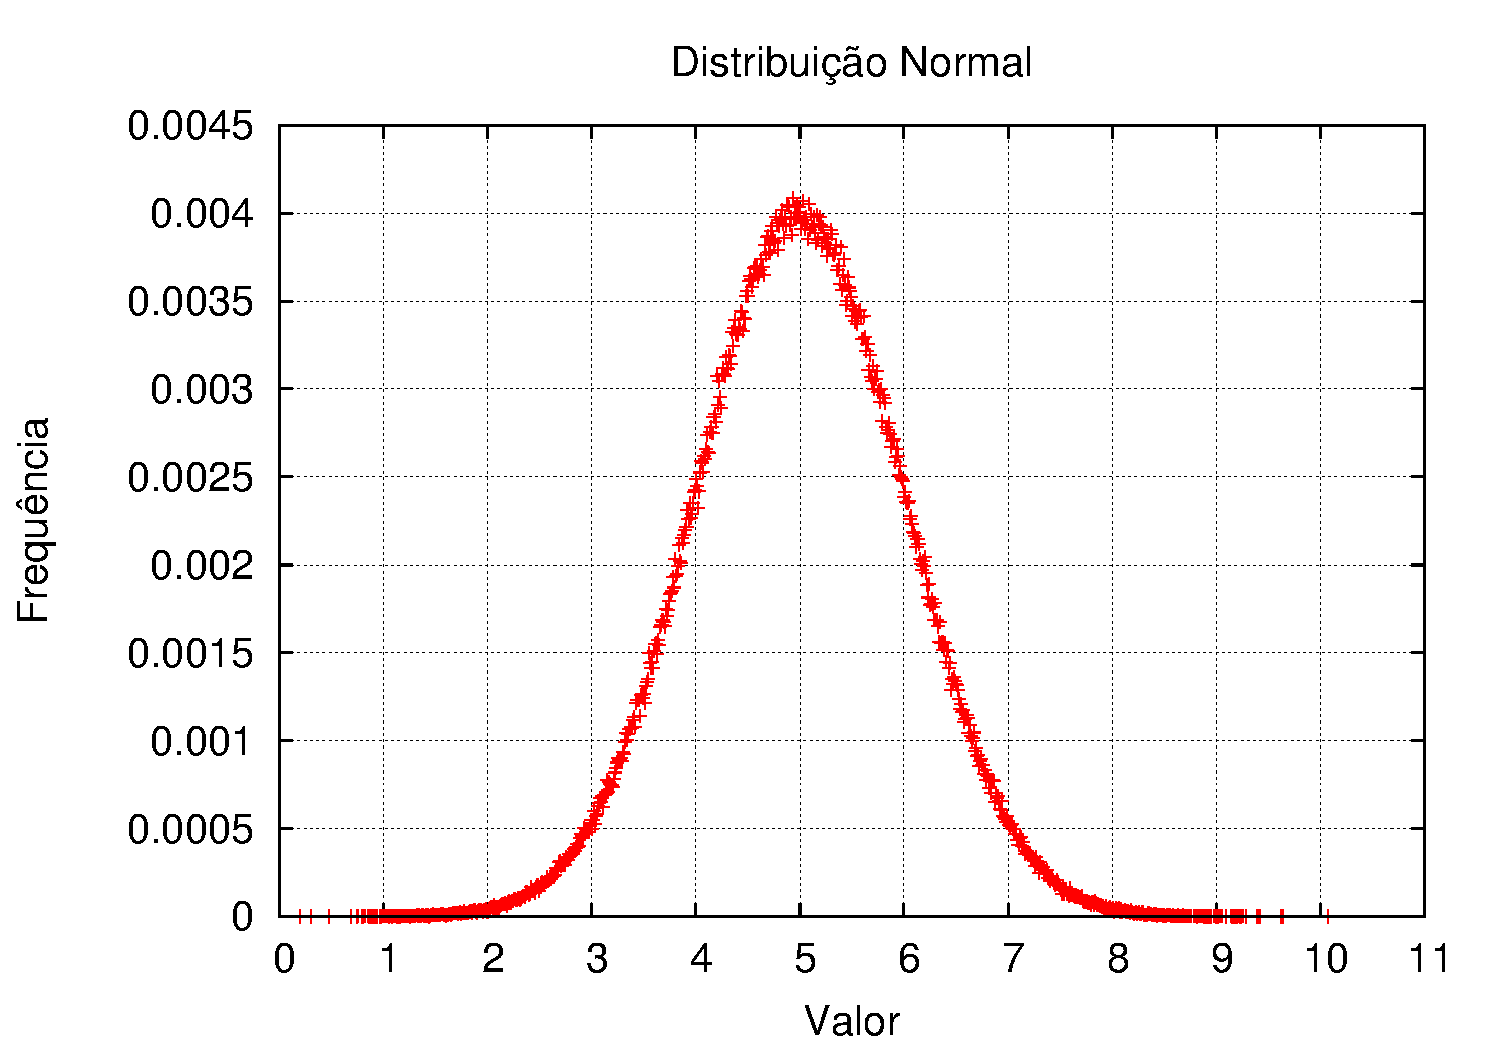
\includegraphics[width=0.3\textwidth]{figuras/DistribuicaoNormal.pdf}
%\caption{Distribuição Normal}
%\label{fig:normal}
%\end{figure}
%
% \begin{figure}
% \centering
%%trim left, bottom, right and top [trim=0cm 2cm 0cm 1cm, width=\textwidth]
%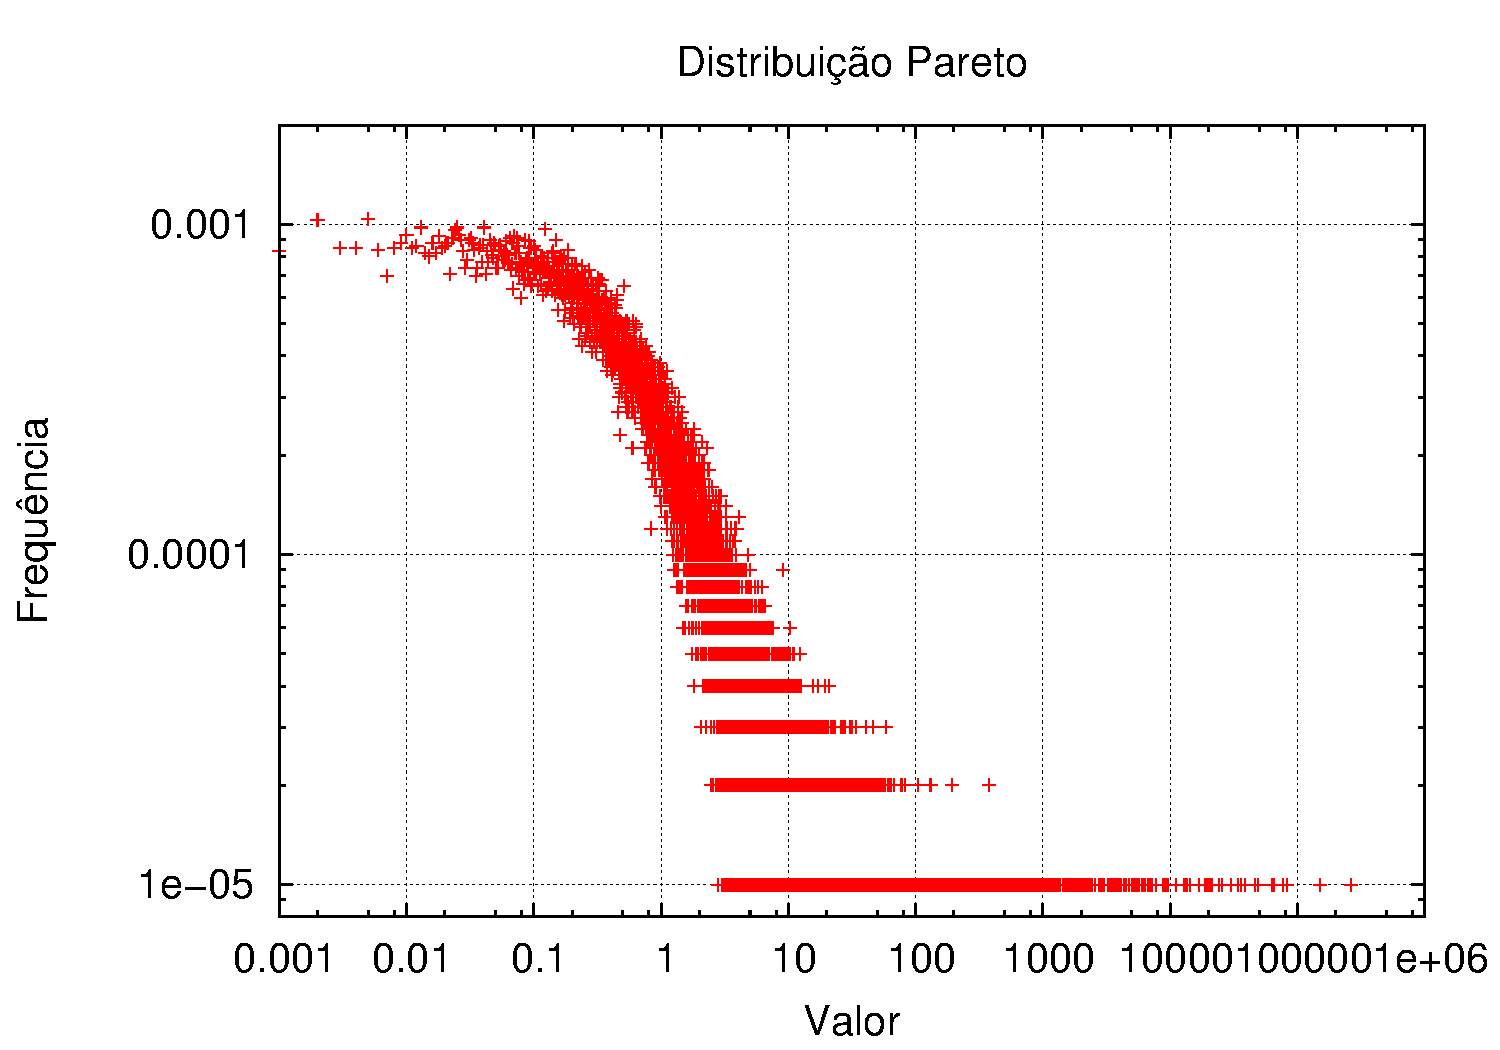
\includegraphics[width=0.3\textwidth]{figuras/DistribuicaoPareto.pdf}
%\caption{Distribuição Pareto}
%\label{fig:pareto}
%\end{figure}

Uma parte fundamental do algoritmo de Ordenação por Amostragem é a definição dos parâmetros de amostragem de chaves, para uma amostragem que resulte em partições balanceadas. Nos testes realizados, os parâmetros definidos foram o número máximo de amostras e o número de partições para cada caso.  O número máximo de amostras foi fixado em 10 mil, e o número de partições foi função do número de máquinas utilizadas e núcleos dos processadores: \mbox{$ Parti \text{\c{c}} \tilde{o}es = m\acute{a}quinas \times n\acute{u}cleos $}. Dessa forma, para as máquinas utilizadas, que contêm 2 núcleos, obtém-se: 4 partições para 2 máquinas; 6 para 3 máquinas; 8 para 4 máquinas; 10 para 5 máquinas.

A seguir são descritos os três tipos de testes realizados, especificando o número de máquinas utilizadas, o número de arquivos e o tamanho dos arquivos ordenados, assim como os objetivos de avaliação de cada teste.



\subsubsection{Quantidade constante de máquinas e dados} 

Os testes com número constante de máquinas e dados foram realizados em 4 máquinas, com arquivos de $10^{6}$ chaves. Foram feitos testes com 10 conjuntos de dados diferentes e, para cada conjunto, o algoritmo foi executado 10 vezes, com os parâmetros de balanceamento descritos anteriormente.  O objetivo foi avaliar a influência dos valores gerados aleatoriamente no desempenho do algoritmo. 


\subsubsection{Variando a quantidade de dados}
 
 Os testes variando a quantidade de dados também foram executados em 4 máquinas, com conjuntos de dados das três distribuições diferentes. Cada distribuição gerou aleatoriamente uma quantidade de dados entre $10^{6}$ e $10^{10}$. O algoritmo foi executado três vezes em cada conjunto com os parâmetros descritos anteriormente. O objetivo foi avaliar a complexidade do algoritmo quando o tamanho do conjunto de dados a ser ordenado aumenta.
 
\subsubsection{Variando a quantidade de máquinas}

Esses testes foram executados com tamanho constante do arquivo de entrada  ($10^{8}$ chaves) em quantidades de máquinas que variaram de 2 a 5. 
Para cada número de máquinas foram gerados conjuntos com as distribuições diferentes. O algoritmo foi executado três vezes para cada conjunto, com os parâmetros de balanceamento descritos anteriormente. O objetivo foi avaliar a escalabilidade do algoritmo, com diminuição do tempo de ordenação quando se aumenta o número de máquinas.


Os resultados dos testes com quantidade constante de máquinas e dados, variando a quantidade de dados e variando a quantidade de máquinas são apresentados e discutidos no Capítulo \ref{cap:resultados}.


\section{Cronograma de trabalho}


O cronograma de trabalho inclui as tarefas que devem ser realizadas e como elas devem ser alocadas durante as disciplinas TCC I e TCC II para que o projeto possa ser concluído com sucesso.
As atividades a serem desenvolvidas são descritas a seguir:

\begin{num_enum}
 \item \label{c1} Pesquisa bibliográfica sobre o tema do projeto e escrita da proposta.
 \item \label{c2} Estudo detalhado dos algoritmos de ordenação paralela,  modelo MapReduce e Hadoop.
 \item \label{c3} Configuração do ambiente Hadoop no laboratório.
 \item \label{c4} Testes com exemplos do Hadoop e com o algoritmo Ordenação por Amostragem.
 \item \label{c5} Escrita, revisão e entrega do projeto.
 \item \label{c6} Implementação e testes do \textit{Quicksort}.
 \item \label{c7} Análise comparativa dos resultados.
 \item \label{c8} Escrita e revisão do relatório final.
 \item \label{c9} Entrega e apresentação.
 \end{num_enum}
 
 
Na Tabela \ref{tab:cronograma} está descrito o cronograma esperado para o desenvolvimento do projeto. Na disciplina TCC I foram realizadas as atividades 1 a 5, e as demais atividades serão realizadas em TCC II. Cada atividade foi alocada para se adequar da melhor maneira ao tempo disponível, mas é possível que o cronograma seja refinado posteriormente, com a inclusão de novas atividades ou redistribuição das tarefas existentes. 


\begin{table}[h]

\renewcommand{\arraystretch}{1}
\setlength\tabcolsep{3pt}
\begin{center}
\begin{tabular}{| c | c | c | c | c | c | c | c | c | c | c |}
\hline

Atividade &Fev &Mar &Abr &Mai &Jun &Jul &Ago &Set &Out &Nov \\ \hline \hline
\ref{c1}   &$\bullet$ &$\bullet$ & & & & & & & & \\ \hline
\ref{c2}   & &$\bullet$ &$\bullet$ & & & & & & & \\ \hline
\ref{c3}   & & &$\bullet$ & & & & & & & \\ \hline
\ref{c4}   & & &$\bullet$ &$\bullet$ & & & & & & \\ \hline
\ref{c5}   & & & &$\bullet$ &$\bullet$ & & & & & \\ \hline
\ref{c6}   & & & & & &$\bullet$ &$\bullet$ & & & \\ \hline
\ref{c7}   & & & & & & & &$\bullet$ & & \\ \hline
\ref{c8}   & & & & & & & & &$\bullet$ & \\ \hline
\ref{c9}   & & & & & & & & & &$\bullet$ \\ 
\hline
\end{tabular}
\end{center}
\caption{Cronograma proposto para o projeto}
\label{tab:cronograma}
\end{table}
